\textbf{\textit{Soal. }}Let $ABC$ be an acute triangle with circumcircle $\Gamma$. Let $P$ and $Q$ be points in the half plane defined by $BC$ containing $A$, such that $BP$ and $CQ$ are tangents to $\Gamma$ and $PB = BC = CQ$. Let $K$ and $L$ be points on the external bisector of the angle $\angle CAB$ , such that $BK = BA, CL = CA$. Let $M$ be the intersection point of the lines $PK$ and $QL$. Prove that $MK=ML$.

\begin{proof}[\textbf{Solusi. }] (Friday, 23 December 2022) Perhatikan untuk kasus $AB=AC$, karena kesimetrian, jelas bahwa $MK=ML$. Oleh karena itu, WLOG $AB < AC$.
    % \begin{center}
    \begin{asy}
     /* Geogebra to Asymptote conversion, documentation at artofproblemsolving.com/Wiki go to User:Azjps/geogebra */
import graph; size(7cm); 
real labelscalefactor = 0.5; /* changes label-to-point distance */
pen dps = linewidth(0.7) + fontsize(10); defaultpen(dps); /* default pen style */ 
pen dotstyle = black; /* point style */ 
real xmin = -12.234626497306365, xmax = 19.266827063720825, ymin = -5.524367657574273, ymax = 14.054121953014862;  /* image dimensions */
pen ccqqqq = rgb(0.8,0,0); pen qqwuqq = rgb(0,0.39215686274509803,0); pen fuqqzz = rgb(0.9568627450980393,0,0.6); pen zzttff = rgb(0.6,0.2,1); 
 /* draw figures */
draw(circle((-1.76,0.48), 4.7161036864438275), linewidth(0.8)); 
draw((2.823793798727584,1.5892647979790973)--(-6.067812686784653,-1.4394748857086537), linewidth(0.8) + blue); 
draw((-6.067812686784653,-1.4394748857086537)--(2.548971838688842,-1.4368713244961349), linewidth(0.8) + ccqqqq); 
draw((2.823793798727584,1.5892647979790973)--(2.548971838688842,-1.4368713244961349), linewidth(0.8) + qqwuqq); 
draw((-1.7614249705369163,5.1961034711664285)--(2.548971838688842,-1.4368713244961349), linewidth(0.8) + fuqqzz); 
draw((-1.7614249705369163,5.1961034711664285)--(-6.067812686784653,-1.4394748857086537), linewidth(0.8) + zzttff); 
draw((2.823793798727584,1.5892647979790973)--(-1.7585750294630844,-4.2361034711664285), linewidth(0.8)); 
draw((2.548971838688842,-1.4368713244961349)--(5.425273775538271,-0.4571192591524621), linewidth(0.8) + qqwuqq); 
draw((-6.067812686784653,-1.4394748857086537)--(-5.2182465508600355,7.915318930588868), linewidth(0.8) + blue); 
draw((6.051284132561602,6.436043696838606)--(2.548971838688842,-1.4368713244961349), linewidth(0.8) + ccqqqq); 
draw((-9.574881942862403,6.431322251179373)--(-6.067812686784653,-1.4394748857086537), linewidth(0.8) + ccqqqq); 
draw((-9.574881942862403,6.431322251179373)--(6.051284132561602,6.436043696838606), linewidth(0.8) + ccqqqq); 
draw((-9.574881942862403,6.431322251179373)--(-1.7614249705369163,5.1961034711664285), linewidth(0.8) + fuqqzz); 
draw((-1.7614249705369163,5.1961034711664285)--(6.051284132561602,6.436043696838606), linewidth(0.8) + zzttff); 
draw((6.051284132561602,6.436043696838606)--(-6.067812686784653,-1.4394748857086537), linewidth(0.8) + zzttff); 
draw((-9.574881942862403,6.431322251179373)--(2.548971838688842,-1.4368713244961349), linewidth(0.8) + fuqqzz); 
draw((-1.7614249705369163,5.1961034711664285)--(-1.7585750294630844,-4.2361034711664285), linewidth(0.8)); 
draw((-9.574881942862403,6.431322251179373)--(6.549661871501632,11.923810679620285), linewidth(0.8)); 
draw((5.425273775538271,-0.4571192591524621)--(6.549661871501632,11.923810679620285), linewidth(0.8)); 
draw((-5.2182465508600355,7.915318930588868)--(5.425273775538271,-0.4571192591524621), linewidth(0.8)); 
 /* dots and labels */
dot((2.823793798727584,1.5892647979790973),linewidth(1pt) + dotstyle); 
label("$A$", (2.9212452488035967,1.6397560176346972), NE * labelscalefactor); 
dot((-6.067812686784653,-1.4394748857086537),linewidth(1pt) + dotstyle); 
label("$C$", (-6.46711898982766,-2.0328272382486015), W * labelscalefactor); 
dot((2.548971838688842,-1.4368713244961349),linewidth(1pt) + dotstyle); 
label("$B$", (2.662612625149843,-1.9035109264217247), NE * labelscalefactor); 
dot((-9.574881942862403,6.431322251179373),linewidth(1pt) + dotstyle); 
label("$Q$", (-10.03624919624946,6.450322817594511), NE * labelscalefactor); 
dot((6.051284132561602,6.436043696838606),linewidth(1pt) + dotstyle); 
label("$P$", (6.257606093937019,6.269279981036884), NE * labelscalefactor); 
dot((5.425273775538271,-0.4571192591524621),linewidth(1pt) + dotstyle); 
label("$K$", (5.533434747706508,-0.40344170922995487), NE * labelscalefactor); 
dot((-5.2182465508600355,7.915318930588868),linewidth(1pt) + dotstyle); 
label("$L$", (-5.432588495212646,8.079708346613158), NE * labelscalefactor); 
dot((6.549661871501632,11.923810679620285),linewidth(1pt) + dotstyle); 
label("$M$", (6.102426519744767,11.907471176688707), NE * labelscalefactor); 
dot((-1.7614249705369163,5.1961034711664285),linewidth(1pt) + dotstyle); 
label("$T$", (-1.7082787145985934,5.23474948642187), NE * labelscalefactor); 
dot((-1.7585750294630844,-4.2361034711664285),linewidth(1pt) + dotstyle); 
label("$N$", (-2.044501125348473,-4.567426950055385), SE * labelscalefactor); 
dot((-1.756496505723293,-11.115216245908497),linewidth(1pt) + dotstyle); 
label("$D$", (-12.234626497306365,14.054121953014862), NE * labelscalefactor); 
clip((xmin,ymin)--(xmin,ymax)--(xmax,ymax)--(xmax,ymin)--cycle); 
 /* end of picture */
\end{asy}
\end{center}
    \begin{center}
\definecolor{ccqqqq}{rgb}{0.8,0,0}
\definecolor{qqwuqq}{rgb}{0,0.39215686274509803,0}
\definecolor{fuqqzz}{rgb}{0.9568627450980393,0,0.6}
\definecolor{zzttff}{rgb}{0.6,0.2,1}
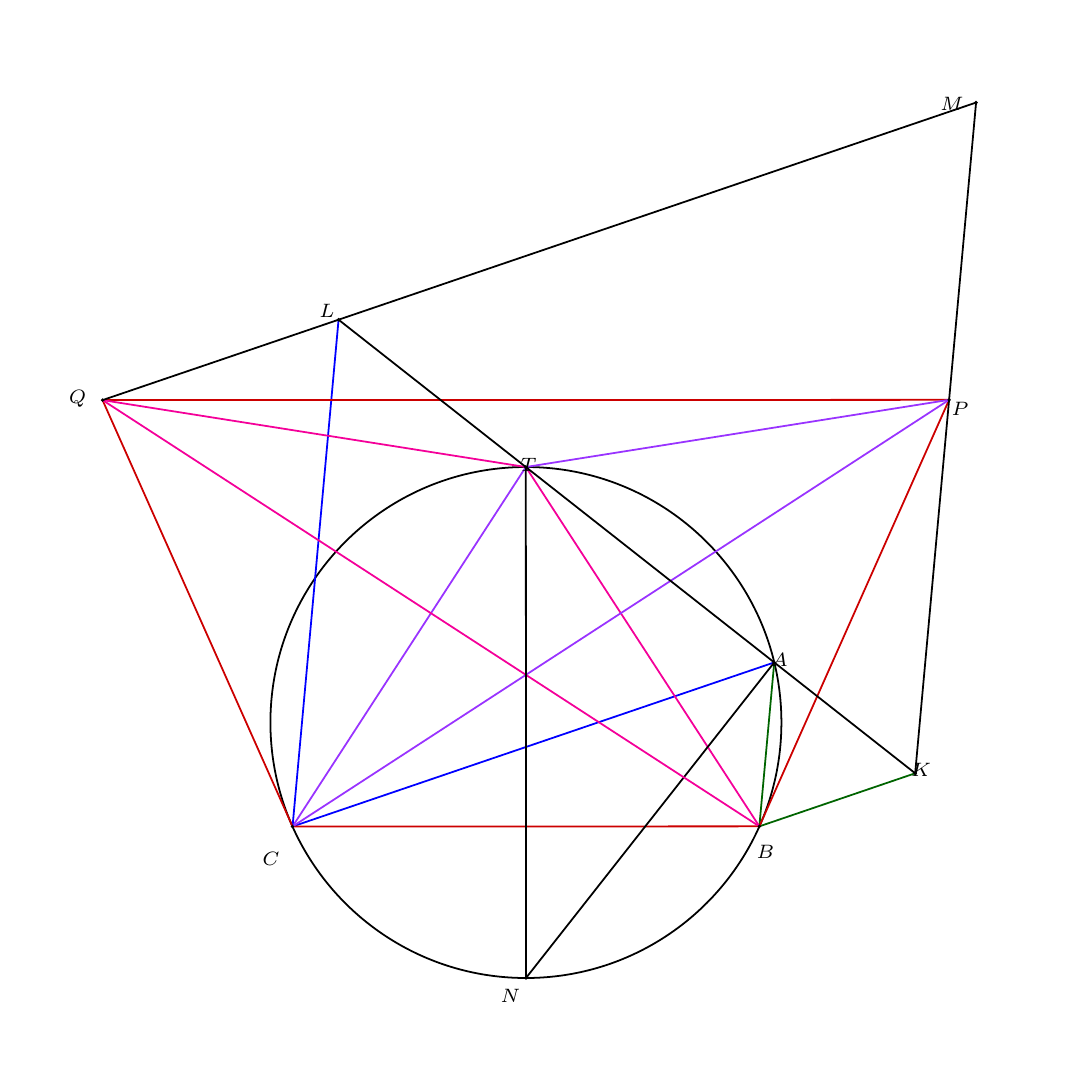
\begin{tikzpicture}[line cap=round,line join=round,scale=0.688]
\clip(-10.9572,-5.5244) rectangle (7.9320,13.3062);
\draw [line width=0.64pt] (-1.76000,0.48000) circle (4.7161036864438275cm);
\draw [line width=0.64pt,color=blue] (2.82379,1.58926) -- (-6.06781,-1.43947);
\draw [line width=0.64pt,color=ccqqqq] (-6.06781,-1.43947) -- (2.54897,-1.43687);
\draw [line width=0.64pt,color=qqwuqq] (2.82379,1.58926) -- (2.54897,-1.43687);
\draw [line width=0.64pt,color=fuqqzz] (-1.76142,5.19610) -- (2.54897,-1.43687);
\draw [line width=0.64pt,color=zzttff] (-1.76142,5.19610) -- (-6.06781,-1.43947);
\draw [line width=0.64pt] (2.82379,1.58926) -- (-1.75858,-4.23610);
\draw [line width=0.64pt,color=qqwuqq] (2.54897,-1.43687) -- (5.42527,-0.45712);
\draw [line width=0.64pt,color=blue] (-6.06781,-1.43947) -- (-5.21825,7.91532);
\draw [line width=0.64pt,color=ccqqqq] (6.05128,6.43604) -- (2.54897,-1.43687);
\draw [line width=0.64pt,color=ccqqqq] (-9.57488,6.43132) -- (-6.06781,-1.43947);
\draw [line width=0.64pt,color=ccqqqq] (-9.57488,6.43132) -- (6.05128,6.43604);
\draw [line width=0.64pt,color=fuqqzz] (-9.57488,6.43132) -- (-1.76142,5.19610);
\draw [line width=0.64pt,color=zzttff] (-1.76142,5.19610) -- (6.05128,6.43604);
\draw [line width=0.64pt,color=zzttff] (6.05128,6.43604) -- (-6.06781,-1.43947);
\draw [line width=0.64pt,color=fuqqzz] (-9.57488,6.43132) -- (2.54897,-1.43687);
\draw [line width=0.64pt] (-1.76142,5.19610) -- (-1.75858,-4.23610);
\draw [line width=0.64pt] (-9.57488,6.43132) -- (6.54966,11.92381);
\draw [line width=0.64pt] (5.42527,-0.45712) -- (6.54966,11.92381);
\draw [line width=0.64pt] (-5.21825,7.91532) -- (5.42527,-0.45712);
\begin{scriptsize}
\fill (2.823793798727584,1.5892647979790973) circle (1pt);
\fill (-6.067812686784653,-1.4394748857086537) circle (1pt);
\fill (2.548971838688842,-1.4368713244961349) circle (1pt);
\fill (-9.574881942862403,6.431322251179373) circle (1pt);
\fill (6.051284132561602,6.436043696838606) circle (1pt);
\fill (5.425273775538271,-0.4571192591524621) circle (1pt);
\fill (-5.2182465508600355,7.915318930588868) circle (1pt);
\fill (6.549661871501632,11.923810679620285) circle (1pt);
\fill (-1.7614249705369163,5.1961034711664285) circle (1pt);
\fill (-1.7585750294630844,-4.2361034711664285) circle (1pt);
\fill (-1.756496505723293,-11.115216245908497) circle (1pt);
\node at (2.9212452488035967,1.6397560176346972) {$A$};
\node at (-6.46711898982766,-2.0328272382486015) {$C$};
\node at (2.662612625149843,-1.9035109264217247) {$B$};
\node at (-10.03624919624946,6.450322817594511) {$Q$};
\node at (6.257606093937019,6.269279981036884) {$P$};
\node at (5.533434747706508,-0.40344170922995487) {$K$};
\node at (-5.432588495212646,8.079708346613158) {$L$};
\node at (6.102426519744767,11.907471176688707) {$M$};
\node at (-1.7082787145985934,5.23474948642187) {$T$};
\node at (-2.044501125348473,-4.567426950055385) {$N$};
\node at (-12.234626497306365,14.054121953014862) {$D$};
\end{scriptsize}
\end{tikzpicture}
\end{center}

Misalkan  $T \neq A$ adalah perpotongan garis bagi luar $\angle BAC$ dengan lingkaran $\Gamma$. Lalu, misalkan $N \neq A$ adalah perpotongan garis bagi dalam $\angle BAC$ dengan lingkaran $\Gamma$.
Dari sifat garis bagi dalam dan luar, $\angle TAN = 90^\circ$ yang menunjukkan juga bahwa $TN$ diameter $\Gamma$. Selain itu, $T$ adalah titik tengah dari busur $BC$ sehingga $TB=TC$. . 

\begin{lemmarev}
    $TQCB$ dan $TPBC$ adalah layang-layang yang kongruen
    \begin{proof}[\textbf{Bukti.}]
        Karena $QC$ menyinggung $\Gamma$ di $C$, maka $\angle TCQ = \angle TBC = \angle BCT$. Di lain sisi, karena $BC=CQ$ dan $TB=TC \implies \angle TBC = \angle BCT$, maka $TC \perp QB$ sehingga $TQCB$ adalah layang-layang dengan $TB=TQ$. Analogi cara tersebut, didapatkan bahwa $TPBC$ adalah layang-layang juga.

        Selanjutnya, karena $TN$ adalah garis sumbu yang membagi dua sama besar segmen $BC$ dan $TN \perp BC$, serta $BP=CQ$, maka dari kesimetrian kita punya $TQ=TP$ dan $TC=TB$. Hal ini menyebabkan $TQCB \cong TPBC$.    \end{proof}
\end{lemmarev}

\begin{lemmarev}
    $LQTC$ dan $PKTB$ adalah segiempat siklis.
    \begin{proof}[\textbf{Bukti.}]
        Perhatikan bahwa $\angle TLC = \angle CAT$ karena $LC = AC$. Dari sini, karena $TQCB \cong TPBC$ adalah layang-layang dan $TABC$ siklis, maka
        $$\angle TLC = \angle CAT = \angle CBT = \angle TQC$$
        yang menunjukkan bahwa $LQTC$ siklis. Dengan cara serupa didapat $PKTB$ siklis.
    \end{proof}
\end{lemmarev}

Karena layang-layang $TQCB$ dan $TPBC$ kongruen, maka $\angle TCQ = \angle PBT$. Berarti akan didapat
\begin{align*}
    \angle KLM = 180^\circ - \angle QLT = \angle TCQ = \angle PBT = \angle PKT = \angle MKL
\end{align*}
yang membuktikan bahwa $ML=MK$.

\end{proof}